%%% LaTeX Template: Article/Thesis/etc. with colored headings and special fonts
%%%
%%% Source: http://www.howtotex.com/
%%% Feel free to distribute this template, but please keep to referal to http://www.howtotex.com/ here.
%%% February 2011
%%%
%%% Modified January 2016 by CDM

%%%  Preamble
\documentclass[11pt,letterpaper]{article}
\usepackage[margin=1.0in]{geometry}
\usepackage[T1]{fontenc}
\usepackage[bitstream-charter]{mathdesign}
\usepackage[latin1]{inputenc}					
\usepackage{amsmath}						
\usepackage{xcolor}
\usepackage{cite}
\usepackage{hyphenat}
\usepackage{graphicx}
\usepackage{float}
\usepackage{subfigure}
\usepackage{sectsty}
\usepackage[compact]{titlesec} 
\usepackage[tablegrid]{vhistory}
\usepackage{pbox}
\allsectionsfont{\color{accentcolor}\scshape\selectfont}

%%% Definitions
\definecolor{accentcolor}{rgb}{0.0,0.0,0.5} 
\newcommand{\teamname}{Team Telepresence}
\newcommand{\productname}{Rift Telepresence}
\newcommand{\coursename}{CSE 4317: Senior Design II}
\newcommand{\semester}{Spring 2017}
\newcommand{\docname}{Detailed Design Specification}
\newcommand{\department}{Department of Computer Science \& Engineering}
\newcommand{\university}{The University of Texas at Arlington}
\newcommand{\authors}{Cameron Adams \\ John Green \\ Andy Le \\ Clement Olayiwola \\ Ty Simmel}

%%% Headers and footers
\usepackage{fancyhdr}
	\pagestyle{fancy}						% Enabling the custom headers/footers
\usepackage{lastpage}	
	% Header (empty)
	\lhead{}
	\chead{}
	\rhead{}
	% Footer
	\lfoot{\footnotesize \teamname \ - \semester}
	\cfoot{}
	\rfoot{\footnotesize page \thepage\ of \pageref{LastPage}}	% "Page 1 of 2"
	\renewcommand{\headrulewidth}{0.0pt}
	\renewcommand{\footrulewidth}{0.4pt}

%%% Change the abstract environment
\usepackage[runin]{abstract}			% runin option for a run-in title
%\setlength\absleftindent{30pt}			% left margin
%\setlength\absrightindent{30pt}		% right margin
\abslabeldelim{\quad}	
\setlength{\abstitleskip}{-10pt}
\renewcommand{\abstractname}{}
\renewcommand{\abstracttextfont}{\color{accentcolor} \small \slshape}	% slanted text

%%% Start of the document
\begin{document}

%%% Cover sheet
{\centering \huge \color{accentcolor} \sc \textbf{\department \\ \university} \par}
\vspace{1 in}
{\centering \huge \color{accentcolor} \sc \textbf{\docname \\ \coursename \\ \semester} \par}
\vspace{0.5 in}
\begin{figure}[h!]
	\centering
   	
\includegraphics[width=0.60\textwidth]{images/test_image}
\end{figure}
\vspace{0.5 in}
{\centering \huge \color{accentcolor} \sc \textbf{\teamname \\ \productname} \par}
\vspace{0.5 in}
{\centering \large \sc \textbf{\authors} \par}
\newpage


%\vspace{1 in}
%\centerline{January 13th, 2012}
%\newpage

%%% Revision History
\begin{versionhistory}
  	\vhEntry{0.1}{02.26.2017}{CA|JG|AL|CO|TS}{Document creation}
  	\vhEntry{0.2}{03.10.2017}{CA|JG|AL|CO|TS}{Update document}
  	\vhEntry{0.3}{05.08.2017}{CA|JG|AL|CO|TS}{Update document with new design}
  	%\vhEntry{1.0}{1.20.2016}{AT|GH|CB}{official release}
  	%\vhEntry{1.1}{1.31.2016}{AL}{added design review requests}
\end{versionhistory}
\newpage

%%% Table of contents
\setcounter{tocdepth}{2}
\tableofcontents
\newpage

%%% List of figures and tables (optional)
\listoffigures
\listoftables
\newpage

%%% Document sections
\section{Introduction}
The project will be a custom stereoscopic camera mounted on a gimbal with 3D movement capabilites (pitch, yaw, roll). The movement of the cameras will be one-to-one with the movement of a virtual reality headset on the user. Minimal computation will be used onboard the actual unit. The majority of processing will be accomplished by the computer running the virtual reality headset. Camera focal points will be preset and calibrated to predetermine the focal distance. Initial versions of the system will use a wire tether for data transfer between the camera unit and processing unit.
\section{System Overview}
The Camera System handles three primary tasks. The motor controller board receives signals from the Processing System. The control board then orients the gimbal to the angles specified by the signals. For the final task, the cameras capture stereo video and pass the video to the Processing System. The Processing System serves as an intermediary between the Camera System and Virtual Reality System. The two functionalities are processing the video and translating the head tracking data. The final system is the Virtual Reality System. This system is responsible for the stereo display of the video and the capture of the raw head tracking data.

\begin{figure}[h!]
	\centering
 	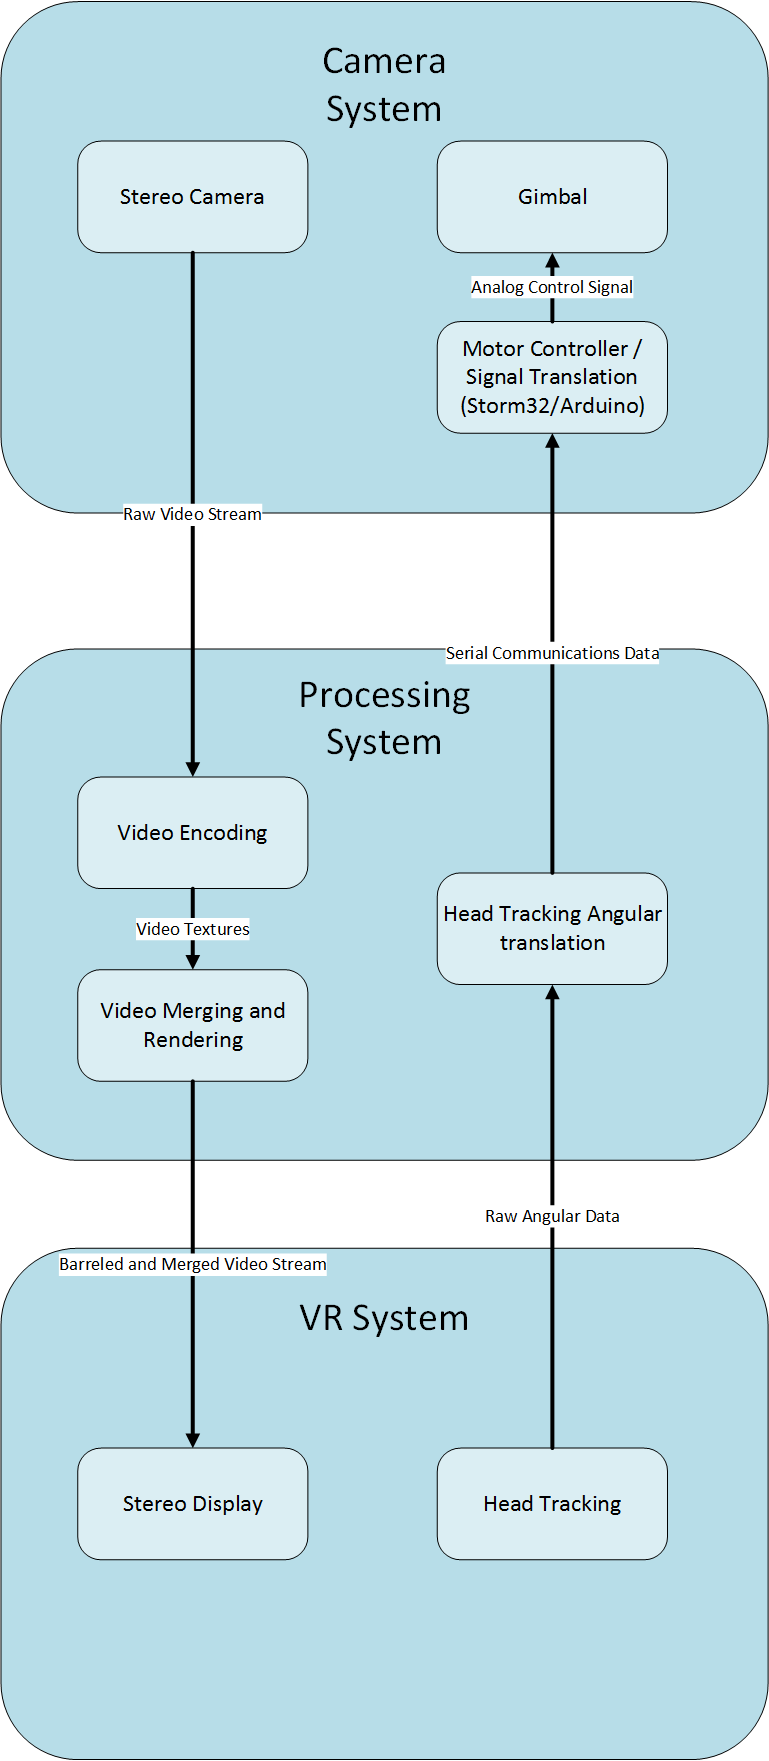
\includegraphics[width=0.27\textwidth]{images/Overview}
 \caption{System architecture}
\end{figure}

\newpage
\section{Camera System Layer Subsystems}
The Camera System Layer contains a camera subsystem, the gimbal subsystem, and signal controller subsystem. The camera subsystem streams the raw video feeds of the stereo cameras. The gimbal subsystem maintains the desired camera angles. The signal controller subsystem receives the angular data and controls the motor based on the data.

\begin{figure}[h!]
	\centering
 	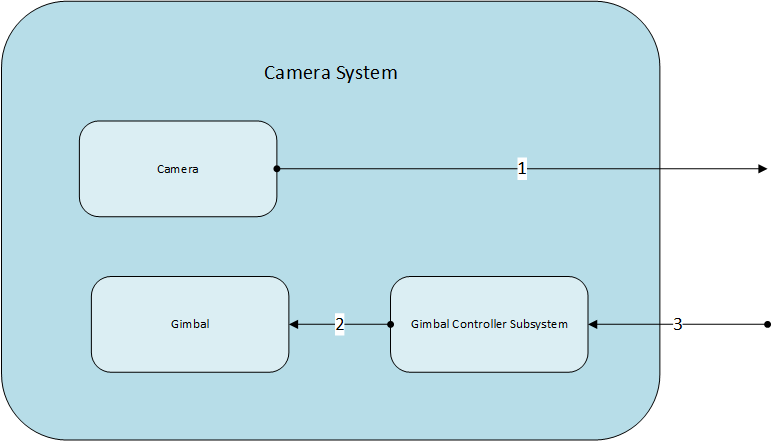
\includegraphics[width=0.60\textwidth]{images/camerasubsystem}
 \caption{Camera System Layer subsystem description diagram}
\end{figure}

\subsection{Layer Hardware}
The Camera System has many hardware components. The camera subsystem contains two wide-angle HD USB camera modules, ELP-USBFHD01M-L21. The gimbal subsystem contains three brushless motors, Rctimer GBM2804, and a custom 3D printed housing. The signal controller subsystem contains a motor control board, Storm32-BGC V1.3.

\subsection{Layer Operating System}
Windows 7 or newer

\subsection{Layer Software Dependencies}
Requires the width and height of the video resolution to be set before the cameras begin to start sending video feed.

\subsection{Camera Subsystem}
The camera subsystem receives input from the cameras and sends the video signal to the Processing System.

\subsubsection{Subsystem Hardware}
The camera modules mentioned above (model No: ELP-USBFHD01M-L21) will be used side-by-side, separated by about 65 mm to simulate the average distance between human eyes.

\subsubsection{Subsystem Operating System}
Supporting operating system: WinXP, Vista, Win7, Win8, Linux with UVC MAC-OS X 10.4.8 or later, Wince with UVC, Android 4.0 or above

\subsubsection{Subsystem Software Dependencies}
The video resolution of the cameras is required to be set before starting to send video feed to the video encoding subsystem in the Processing System.

% Anything?
\subsubsection{Subsystem Programming Languages}
None

\subsubsection{Subsystem Data Structures}
The video output of the camera modules is FMPEG with a user-specified frame rate and resolution per frame.

% Anything?
\subsubsection{Subsystem Data Processing}
None

\subsection{Gimbal Subsystem}
The gimbal subsystem is a custom built three axis gimbal with stereo camera mounts and external mounting plates.

\subsubsection{Subsystem Hardware}
There are three Rctimer GBM2804 motors and a custom 3D printed housing.

% Anything?
\subsubsection{Subsystem Operating System}
None

\subsubsection{Subsystem Software Dependencies}
The Rctimer motors rely on the PWM output of the Storm32-BGC board for angular instruction.

% Anything?
\subsubsection{Subsystem Programming Languages}
None

% Anything?
\subsubsection{Subsystem Data Structures}
None

% Anything?
\subsubsection{Subsystem Data Processing}
None

\subsection{Signal Controller Subsystem}
The signal controller subsystem receives a pulse width modulated signal representing the three angles that the camera should be aligned relative to the initialized position. This alignment is achieved through the use of two inertial measurement unit modules. The control board adjusts the motors to keep the gimbal in alignment.

\subsubsection{Subsystem Hardware}
There are three Rctimer GBM2804 motors, a custom 3D printed housing, a Storm32-BGC V1.3, and MPU6050 IMU.

\subsubsection{Subsystem Operating System}
The control board runs on configurable firmware. The version used was V0.90.

\subsubsection{Subsystem Software Dependencies}
The PWM signal must be a pulse between 1-2 ms with a 15ms period.

\subsubsection{Subsystem Programming Languages}
User specifications can be digitally sent to the Storm32-BGC board using OlliW's custom user interface which translates settings directly to assembly level programming of the onboard STM32F103RC MCU.

\subsubsection{Subsystem Data Structures}
The Storm32-BGC v1.3 utilizes a Futuba S-Bus for data communication across the board's components.

% Anything?
\subsubsection{Subsystem Data Processing}
None
\newpage
\section{Processing System Layer Subsystems}
This system contains the video encoding subsystem, video rendering subsystem, and the head tracking translation subsystem. The subsystems communicate with the Camera System and the Virtual Reality System respectively. Video data will be received from the Camera System and rendered to the Virtual Reality System. The raw head tracking data is captured and translated to analog signals for the Camera System.

\begin{figure}[h!]
	\centering
 	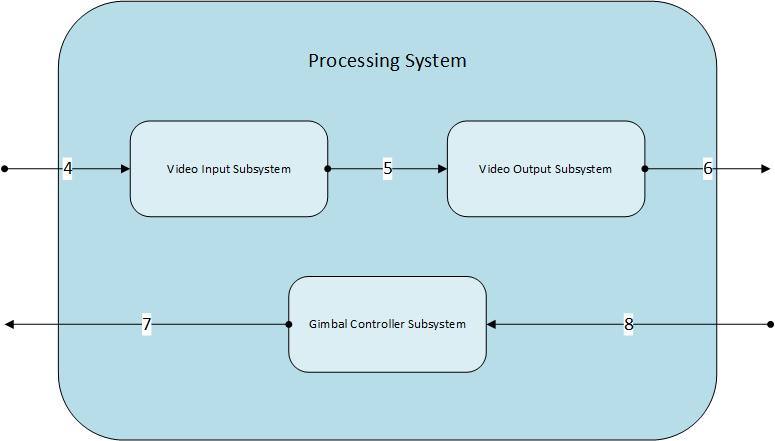
\includegraphics[width=0.60\textwidth]{images/processingsubsystem}
 \caption{Processing System Layer subsystem description diagram}
\end{figure}

\subsection{Layer Hardware}
A computer powerful enough to encode and render two 1080p 30 frames per second video, an Intel i5 or an Nvidia GeForce GTX 970 are the suggested minimums, and an Arduino Uno is used as the serical interface for the Storm32-BGC gimbal controller.

\subsection{Layer Operating System}
The supported operating system is Windows 7 or newer.

\subsection{Layer Software Dependencies}
An Oculus Rift setup utility has been executed on the computer. Unity 5.5 if cameras need to be adjusted or changes are needed. Arduino IDE is recommended if serial interface changes must be made as well as for the initial setup of the Arduino Uno.

\subsection{Video Encoding Subsystem}
This subsystem receives the raw FMPEG video streams from the Camera System. The raw video is encoded into a Unity texture.

\subsubsection{Subsystem Hardware}
A minimum of Intel i5 or Nvidia GeForce GTX 970 is suggested.

\subsubsection{Subsystem Operating System}
Windows 7 or newer

\subsubsection{Subsystem Software Dependencies}
Unity 5.5

\subsubsection{Subsystem Programming Languages}
C\# has been used as the default scripting language for its nativity in Unity.

\subsubsection{Subsystem Data Structures}
Array of textures and video frame buffers.

\subsubsection{Subsystem Data Processing}
FMPEG to Unity texture

\subsection{Video Rendering Subsystem}
This subsystem takes the two video textures and overlays them onto a user interface menu element. Then, the images are barreled and merged. The rendered image is streamed to the Virtual Reality System.

\subsubsection{Subsystem Hardware}
A minimum of Intel i5 or Nvidia GeForce GTX 970 is suggested.

\subsubsection{Subsystem Operating System}
Windows 7 or newer

\subsubsection{Subsystem Software Dependencies}
Unity 5.5

\subsubsection{Subsystem Programming Languages}
C\#

% Anything?
\subsubsection{Subsystem Data Structures}
None

\subsubsection{Subsystem Data Processing}
For each frame of the videos, barreled distortion is applied to match the perspective of the Oculus Rift. Each camera input is applied to its respective eye's texture to create the illusion of depth.

\subsection{Angular Translation Subsystem}
This subsystem takes the raw head tracking data and converts it into angular data. The angular data will then be sent to an Arduino over a serial interface. The Arduino converts the data to a PWM readable signal and sends that signal to the gimbal subsystem of the Camera System.

\subsubsection{Subsystem Hardware}
Arduino Uno

\subsubsection{Subsystem Operating System}
Arduino IDE

\subsubsection{Subsystem Software Dependencies}
Unity 5.5

\subsubsection{Subsystem Programming Languages}
C

\subsubsection{Subsystem Data Structures}
The `Servo.h' library has been utilized to easily translate integer values into PWM readable signals to be written out from the Arduino.

\subsubsection{Subsystem Data Processing}
At sixty times a second, the system reads the head tracking data and converts it to angular data. The conversion uses the x-y-z position values to generate euler angles. The angles are modified to conform to the system operational ranges.
\newpage
\section{Virtual Reality System Layer Subsystems}
The Virtual Reality System is focused on delivering real-time video and tracking of the head movement on the virtual reality headset. This system contains the stereo display subsystem and the head tracking subsystem. The stereo display subsystem will interact with the video rendering subsystem, while the head tracking subsystem will interact with the angular translation subsystem.

\begin{figure}[h!]
	\centering
 	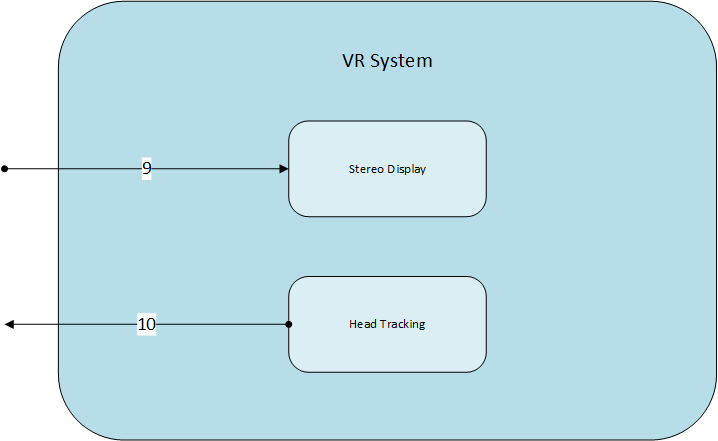
\includegraphics[width=0.60\textwidth]{images/vrsubsystem}
 \caption{Example subsystem description diagram}
\end{figure}

\subsection{Layer Hardware}
The Oculus Rift headset and the Oculus positional sensor are used in this system.

\subsection{Layer Operating System}
Windows 7 or newer

\subsection{Layer Software Dependencies}
Oculus Rift drivers and utilities

\subsection{Stereo Display Subsystem}
This subsystem interacts with the video rendering subsystem of the Processing System by receiving video data. This subsystem decodes and displays the video feed from the video rendering subsystem.

\subsubsection{Subsystem Hardware}
Oculus Rift headset

% Anything?
\subsubsection{Subsystem Operating System}
None

\subsubsection{Subsystem Software Dependencies}
Oculus Rift drivers and utilities are installed on the computer.

% Anything?
\subsubsection{Subsystem Programming Languages}
None

% Anything?
\subsubsection{Subsystem Data Structures}
None

% Anything?
\subsubsection{Subsystem Data Processing}
None

\subsection{Head Tracking Subsystem}
This subsystem interacts with the angular translation subsystem of the Processing System by sending positional data gathered from the gyros and accelerometers in the Oculus headset combined with the Oculus positional sensor.

\subsubsection{Subsystem Hardware}
Oculus Rift headset and Oculus positional sensor

% Anything?
\subsubsection{Subsystem Operating System}
None

\subsubsection{Subsystem Software Dependencies}
Unity 5.5, Oculus Rift drivers, and Oculus Rift utilities are installed on the computer.

% Anything?
\subsubsection{Subsystem Programming Languages}
None

% Anything?
\subsubsection{Subsystem Data Structures}
None

% Anything?
\subsubsection{Subsystem Data Processing}
None
\newpage
\section{Appendix A}
Include any additional documents (CAD design, circuit schematics, etc) as an appendix as necessary.
\newpage

%%% References
\bibliographystyle{plain}
\bibliographystyle{reference/IEEEtran_custom}
\bibliography{reference/refs}{}

\end{document}